\documentclass[11pt,a4paper]{article}
\usepackage{amsmath,amsthm,amsfonts,amssymb,amscd}
\usepackage{enumerate} 
\usepackage{physics}
\usepackage{enumerate}
\usepackage{fancyhdr}
\usepackage{hyperref}
\usepackage{graphicx}
\hypersetup{colorlinks,
    linkcolor=blue,
    citecolor=blue,      
    urlcolor=blue
}
\usepackage{xurl}

\oddsidemargin0.1cm 
\evensidemargin0.8cm
\textheight22.7cm 
\textwidth15cm \topmargin-0.5cm

\newtheorem{theorem}{Theorem}
\newtheorem{corollary}{Corollary}
\newtheorem{lemma}{Lemma}
\newtheorem{proposition}{Proposition}

\theoremstyle{definition}
\newtheorem{remark}{Remark}
\newtheorem{definition}{Definition}
\newtheorem{observation}{Observation}
\newtheorem{note}{Note}
\newtheorem{hope}{Hope}
\newtheorem{warning}{Warning}
\newtheorem{problem}{Problem}
\newtheorem{fear}{Fear}
\newtheorem{question}{Question}

\newcommand{\Z}{\mathbb{Z}}
\newcommand{\R}{\mathbb{R}}
\newcommand{\C}{\mathbb{C}}
\newcommand{\Q}{\mathbb{Q}}
\newcommand{\A}{\mathbb{A}}

\usepackage{listings}
\usepackage{xcolor}

\definecolor{codegreen}{rgb}{0,0.6,0}
\definecolor{codegray}{rgb}{0.5,0.5,0.5}
\definecolor{codepurple}{rgb}{0.58,0,0.82}
\definecolor{backcolour}{rgb}{0.95,0.95,0.92}

\lstdefinestyle{mystyle}{
    backgroundcolor=\color{backcolour},   
    commentstyle=\color{codegreen},
    keywordstyle=\color{magenta},
    numberstyle=\tiny\color{codegray},
    stringstyle=\color{codepurple},
    basicstyle=\ttfamily\footnotesize,
    breakatwhitespace=false,         
    breaklines=true,                 
    captionpos=b,                    
    keepspaces=true,                 
    numbers=left,                    
    numbersep=5pt,                  
    showspaces=false,                
    showstringspaces=false,
    showtabs=false,                  
    tabsize=2
}

\lstset{style=mystyle}

\newcommand{\MultiSet}{\mathrm{MultiSet}}
\newcommand{\len}{\mathrm{len}}
\newcommand{\din}{\texttt{d\_in}}
\newcommand{\dout}{\texttt{d\_out}}
\newcommand{\T}{\texttt{T} }
\newcommand{\Relation}{\texttt{Relation}}
\newcommand{\X}{\mathcal{X}}
\newcommand{\Y}{\mathcal{Y}}
\newcommand{\True}{\texttt{True}}
\newcommand{\False}{\texttt{False}}
\newcommand{\clamp}{\texttt{clamp}}
\newcommand{\function}{\texttt{function}}
\newcommand{\float}{\texttt{float }}
\newcommand{\questionc}[1]{\textcolor{red}{\textbf{Question:} #1}}

\newcommand{\silvia}[1]{{ {\color{blue}{(silvia)~#1}}}}
\newcommand{\grace}[1]{{ {\color{purple}{(grace)~#1}}}}
\newcommand{\connor}[1]{{ {\color{teal}{(connor)~#1}}}}
\newcommand{\mike}[1]{{ {\color{green}{(mike)~#1}}}}
\newcommand{\todo}{{\textcolor{red}{TODO }}}


\title{Privacy Proofs for OpenDP: Clamping II}
\author{S\'ilvia Casacuberta}
\date{Summer 2021}

\begin{document}

\maketitle

\tableofcontents

\section{Algorithm Implementation}
\subsection{Code in Rust}
The current OpenDP library contains the \texttt{make\_clamp} function implementing the clamping function for both the symmetric distance (with vectors) and the absolute distance (with elements) cases. In this proof, we deal with the clamping with absolute distance constructor. This is defined in lines 25-38 of the file \texttt{clamp.rs} in the Git repository\footnote{We refrain from using the clampable domain that is used in the pseudocode.} (\url{https://github.com/opendp/opendp/blob/main/rust/opendp/src/trans/clamp.rs#L46-L72}).

\begin{figure}[ht]
    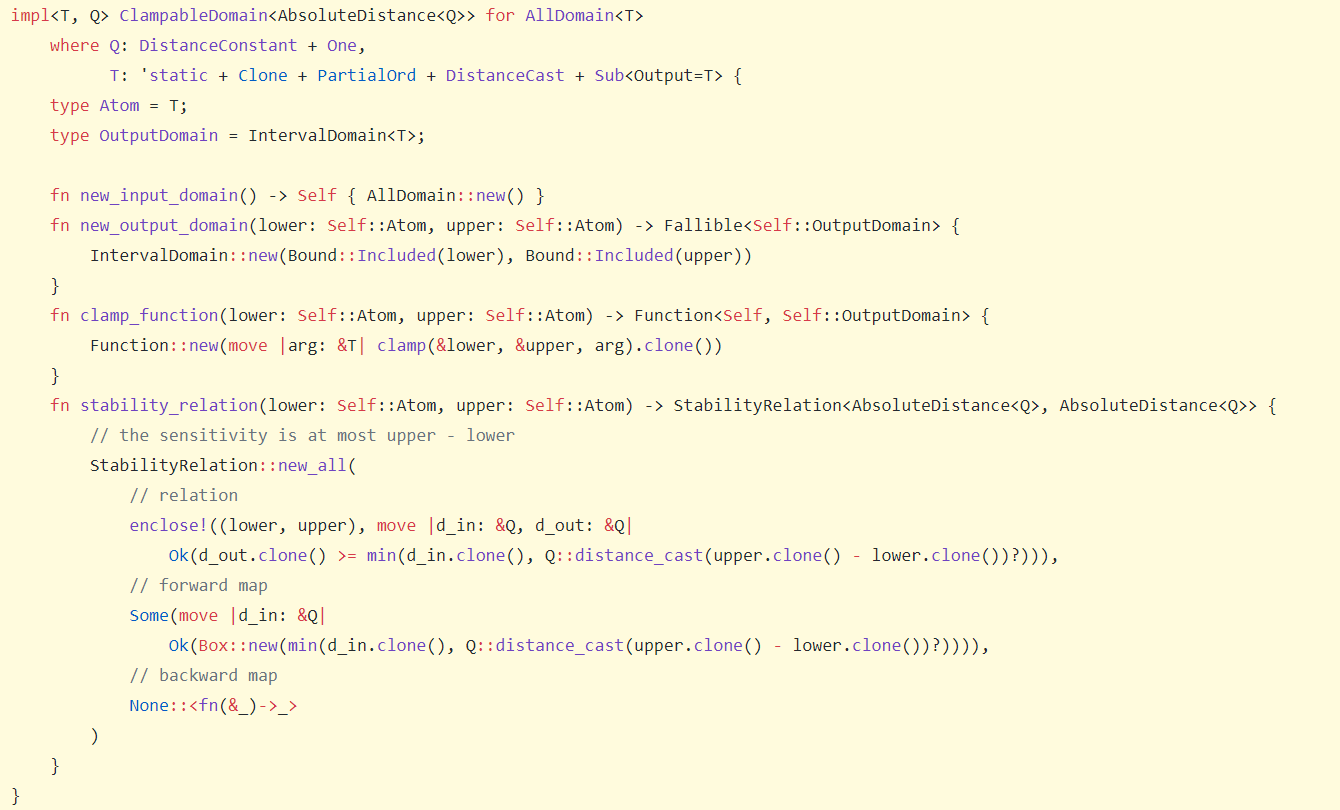
\includegraphics[width=15cm]{abs_clamp_rust.png}
    \centering
    \label{fig:code}
\end{figure}

\silvia{The Rust code shows the \texttt{ClampableDomain} \texttt{impl} for absolute distance instead of the \texttt{pub fn} \texttt{make\_clamp} because it is the part that shows the relevant differences between absolute distance clamping and symmetric distance clamping.}

\subsection{Pseudocode in Python}\label{sec:pseudocode}
We present a simplified Python-like pseudocode of the Rust implementation below. The necessary definitions for the pseudocode can be found at \href{https://www.overleaf.com/project/60d215bf90b337ac02200a99}{``List of definitions used in the pseudocode"}. 

\subsubsection*{Preconditions}
To ensure the correctness of the output, we require the following preconditions:

\begin{itemize}
    \item \textbf{User-specified types:}
    \begin{itemize}
        \item Type \texttt{T} must have traits \texttt{TotalOrd},\footnote{For now, the OpenDP library only implements \texttt{PartialOrd}, but \texttt{TotalOrd} will soon be implemented.} \texttt{DistanceCast}, and \texttt{Sub(Output=T)}.
    \end{itemize}
\end{itemize}

\subsubsection*{Postconditions}
\begin{itemize}
    \item Either a valid \texttt{Transformation} is returned or an error is returned.
\end{itemize}

\begin{lstlisting}[language=Python, escapechar=|] 
def MakeClampAbs(L: T, U: T): |\label{line:def}|
    input_domain = AllDomain(T)
    output_domain = IntervalDomain(L, U) |\label{line:output}|
    input_metric = AbsoluteDistance(Q)
    output_metric = AbsoluteDistance(Q)
    
    def Relation(d_in: Q, d_out: Q) -> bool: |\label{line:rel}|
        return d_out >= min(d_in, U-L)
        
    def function(x: T) -> T: |\label{line:fn}|
        return max(min(x, U), L) |\label{line:return}|
    
    return Transformation(input_domain, output_domain, function, input_metric, output_metric, stability_relation = Relation)
\end{lstlisting}

\section{Proof}
The necessary definitions for the proof can be found at \href{https://www.overleaf.com/project/60d214e390b337703d200982}{``List of definitions used in the proofs"}.

\subsection{Symmetric Distance}
\begin{theorem}
    For every setting of the input parameters \texttt{L, U} to \texttt{MakeClampAbs} such that the given preconditions
    hold, the transformation returned by \texttt{MakeClampAbs} has the following properties:
    \begin{enumerate}
        \item \textup{(Appropriate output domain).} For every element $v$ in \texttt{input\_domain}, $\function(v)$ is in \texttt{output\_domain}.
        
        \item \textup{(Domain-metric compatibility).} The domain \texttt{input\_domain} matches one of the possible domains listed in the definition of \texttt{input\_metric}, and likewise \texttt{output\_domain} matches one of the possible domains listed in the definition of \texttt{output\_metric}.
        
        \item \textup{(Stability guarantee).} For every pair of elements $v, w$ in \texttt{input\_domain} and for every pair $(\din, \dout)$,  where $\din$ is of the associated type for \texttt{input\_metric} and $\dout$ is the associated type for \texttt{output\_metric}, if $v,w$ are $\din$-close under \texttt{input\_metric} and $\Relation(\din, \dout) = \True$, then $\function(v), \function(w)$ are $\dout$-close under \texttt{output\_metric}.
    \end{enumerate}
\end{theorem}

\begin{proof}
\textbf{(Appropriate output domain).} In the case of \texttt{MakeClampAbs}, this corresponds to showing that for every element $x$ of type \texttt{T}, $\function(x)$ is an element of type \texttt{T} and contained in the interval \texttt{[L, U]}. For that, we need to show two things: first, that \texttt{function(x)} has type \texttt{T}. Second, that it belongs to the interval \texttt{[L, U]}.

Firstly, that $\function(x)$ has type \texttt{T} follows from the assumption that element $x$ is in \texttt{input\_domain} and from the type signature of \texttt{function} in line~\ref{line:fn} of the pseudocode (Section~\ref{sec:pseudocode}), which takes in an element of type \texttt{T} and returns an element of type \texttt{T}. If the Rust code compiles correctly, then the type correctness follows from the definition of the type signature enforced by Rust. Otherwise, the code raises an exception for incorrect input type. 

Secondly, we need to show that the vector entries belong to the interval \texttt{[L, U]}. This follows from the definition of \texttt{function} in line \ref{line:fn}. According to line \ref{line:fn} in the pseudocode, there are 3 possible cases to consider:
\begin{enumerate}
    \item \texttt{x} $>$ \texttt{U}: then $\texttt{function(x)}$ returns \texttt{U}.
    \item \texttt{x} $\in$ \texttt{[L, U]}: then $\texttt{function(x)}$ returns \texttt{x}.
    \item \texttt{x} $<$ \texttt{L}: then $\texttt{function(x)}$ returns \texttt{L}.
\end{enumerate}
In all three cases, the returned value of type \T is contained in the interval \texttt{[L, U]}. Hence, the element $\function(x)$ returned in line~\ref{line:return} of the pseudocode is an element of \texttt{output\_domain}.

Lastly, the necessary condition that \texttt{L} $\leq$ \texttt{U} is checked when declaring \texttt{output\_domain = IntervalDomain(L, U)} in line~\ref{line:output} of the pseudocode. This check already exists via the construction of \texttt{IntervalDomain}, which returns an error if \texttt{L} $>$ \texttt{U}. Both \texttt{L} and \texttt{U} have type \texttt{T} by their precondition requirement. Both the definition of \texttt{IntervalDomain} and that of \texttt{function} (line~\ref{line:fn} in the pseudocode, which uses the \texttt{min} and \texttt{max} functions) require that \texttt{T} implements \texttt{TotalOrd}, which holds by the preconditions.

\smallskip
\textbf{(Domain-metric compatibility).}  For \texttt{MakeClampAbs}, this corresponds to showing that both \texttt{AllDomain(T)} and \texttt{IntervalDomain(L, U)} are compatible with absolute distance. The first one follows directly from the definition of absolute distance, as stated in \href{https://www.overleaf.com/project/60d214e390b337703d200982}{``List of definitions used in the proofs"}. The second one follows from the compatibility of absolute distance and \texttt{AllDomain(T)} along with the fact that \texttt{IntervalDomain(L, U)} is a subdomain of \texttt{AllDomain(T)}. By Theorem 2.1 in \href{https://www.overleaf.com/project/60d215bf90b337ac02200a99}{``List of definitions used in the pseudocode"}, this implies that \texttt{IntervalDomain(L, U)} is compatible with absolute distance as well. 
    
\silvia{Flag: this is an example of the subdomain issues that we have been discussing during the week of July 19. Hence this paragraph might need some phrasing updates when the compatibility pairing constructor and the subdomain trait are implemented.}

\smallskip
\textbf{(Stability guarantee).} Throughout the stability guarantee proof, we can assume that $\function(x)$ and $\function(y)$ are in the correct output domain, by the \textit{appropriate output domain property} shown above. 

Since by assumption $\Relation(\din, \dout) = \True$, by the \texttt{MakeClampAbs} stability relation (as defined in line~\ref{line:rel} in the pseudocode), we have that $\dout \geq \min(\din, \texttt{U-L})$. Moreover, $v, w$ are assumed to be $\din$-close. By the definition of the absolute distance metric, this is equivalent to stating that $d_{Abs}(x, y) = |x - y| \leq \din$.

We now consider the values $\function(x)$ and $\function(y)$. There are three possible cases to consider:
\begin{enumerate}
    \item Both $x \in \texttt{[L, U]}$ and $y \in \texttt{[L, U]}$: in this case, $x = \function(x)$ and $y = \function(y)$. Hence, $d_{Abs}(x, y) = |x-y| = |\function(x) - \function(y)|$.
    \item Wlog, $x \in \texttt{[L, U]}$ and $y \notin \texttt{[L, U]}$: if $y < \texttt{L}$ then $y < \function(y) = \texttt{L}$, and if $y > \texttt{U}$, then $y > \function(y) = \texttt{U}$. In both cases, it follows that $|\function(y) - x| < |y - x| = d_{Abs}(x, y)$, since $\function(x) = x$.
    \item Both $x, y \notin \texttt{[L, U]}$: in this case, if both $x, y < \texttt{L}$ or both $x, y > \texttt{U}$, then $|\function(x) - \function(y)| = 0$. Because the absolute value metric is always non-negative, it follows that $|\function(x) - \function(y)| \leq |x - y|$. On the other hand, if $x < \texttt{L}$ and $y > \texttt{U}$ or viceversa, then $|\texttt{U}-\texttt{L}| < |x-y|$. Since by the appropriate domain property we know that $\function(x), \function(y) \in \texttt{[L, U]}$, it follows that $|\function(x) - \function(y)| \leq |\texttt{U}-\texttt{L}|$.
\end{enumerate}

By merging the cases considered above, we conclude that
\[
    d_{Abs}(\function(x), \function(y)) = |\function(x) - \function(y)| \leq 
\]
\[
    \min(|x-y|, \texttt{U-L}) = \min(d_{Abs}(x, y), \texttt{U-L}) \leq \min(\din, \texttt{U-L}).
\]
By the initial assumptions, we recall that $\dout $, and that $x, y$ are $\din$-close. Then,
\[
    d_{Abs}(\function(x), \function(y)) \leq \min(\din, \texttt{U-L}) \leq \dout.
\]
Therefore,
\[
    d_{Abs}(\function(x), \function(y)) \leq \dout,
\]
as we wanted to show.
\end{proof}

\end{document}
